%%%%%%%%%%%%%%%%%%%%%%%%%%%%%%%%%%%%%%%%%
% Wenneker Assignment
% LaTeX Template
% Version 2.0 (12/1/2019)
%
% This template originates from:
% http://www.LaTeXTemplates.com
%
% Authors:
% Vel (vel@LaTeXTemplates.com)
% Frits Wenneker
%
% License:
% CC BY-NC-SA 3.0 (http://creativecommons.org/licenses/by-nc-sa/3.0/)
% 
%%%%%%%%%%%%%%%%%%%%%%%%%%%%%%%%%%%%%%%%%

%----------------------------------------------------------------------------------------
%	PACKAGES AND OTHER DOCUMENT CONFIGURATIONS
%----------------------------------------------------------------------------------------

\documentclass[11pt]{scrartcl} % Font size
\usepackage{graphicx}
%%%%%%%%%%%%%%%%%%%%%%%%%%%%%%%%%%%%%%%%%
% Wenneker Assignment
% Structure Specification File
% Version 2.0 (12/1/2019)
%
% This template originates from:
% http://www.LaTeXTemplates.com
%
% Authors:
% Vel (vel@LaTeXTemplates.com)
% Frits Wenneker
%
% License:
% CC BY-NC-SA 3.0 (http://creativecommons.org/licenses/by-nc-sa/3.0/)
% 
%%%%%%%%%%%%%%%%%%%%%%%%%%%%%%%%%%%%%%%%%

%----------------------------------------------------------------------------------------
%	PACKAGES AND OTHER DOCUMENT CONFIGURATIONS
%----------------------------------------------------------------------------------------

\usepackage{amsmath, amsfonts, amsthm} % Math packages

\usepackage{listings} % Code listings, with syntax highlighting

\usepackage[english]{babel} % English language hyphenation

\usepackage{graphicx} % Required for inserting images
\graphicspath{{Figures/}{./}} % Specifies where to look for included images (trailing slash required)

\usepackage{booktabs} % Required for better horizontal rules in tables

\numberwithin{equation}{section} % Number equations within sections (i.e. 1.1, 1.2, 2.1, 2.2 instead of 1, 2, 3, 4)
\numberwithin{figure}{section} % Number figures within sections (i.e. 1.1, 1.2, 2.1, 2.2 instead of 1, 2, 3, 4)
\numberwithin{table}{section} % Number tables within sections (i.e. 1.1, 1.2, 2.1, 2.2 instead of 1, 2, 3, 4)

\setlength\parindent{0pt} % Removes all indentation from paragraphs

\usepackage{enumitem} % Required for list customisation
\setlist{noitemsep} % No spacing between list items

%----------------------------------------------------------------------------------------
%	DOCUMENT MARGINS
%----------------------------------------------------------------------------------------

\usepackage{geometry} % Required for adjusting page dimensions and margins

\geometry{
	paper=a4paper, % Paper size, change to letterpaper for US letter size
	top=2.5cm, % Top margin
	bottom=3cm, % Bottom margin
	left=3cm, % Left margin
	right=3cm, % Right margin
	headheight=0.75cm, % Header height
	footskip=1.5cm, % Space from the bottom margin to the baseline of the footer
	headsep=0.75cm, % Space from the top margin to the baseline of the header
	%showframe, % Uncomment to show how the type block is set on the page
}

%----------------------------------------------------------------------------------------
%	FONTS
%----------------------------------------------------------------------------------------

\usepackage[utf8]{inputenc} % Required for inputting international characters
\usepackage[T1]{fontenc} % Use 8-bit encoding

\usepackage{fourier} % Use the Adobe Utopia font for the document

%----------------------------------------------------------------------------------------
%	SECTION TITLES
%----------------------------------------------------------------------------------------

\usepackage{sectsty} % Allows customising section commands

\sectionfont{\vspace{6pt}\centering\normalfont\scshape} % \section{} styling
\subsectionfont{\normalfont\bfseries} % \subsection{} styling
\subsubsectionfont{\normalfont\itshape} % \subsubsection{} styling
\paragraphfont{\normalfont\scshape} % \paragraph{} styling

%----------------------------------------------------------------------------------------
%	HEADERS AND FOOTERS
%----------------------------------------------------------------------------------------

%\usepackage{scrlayer-scrpage} % Required for customising headers and footers

%\ohead*{} % Right header
%\ihead*{} % Left header
%\chead*{} % Centre header

%\ofoot*{} % Right footer
%\ifoot*{} % Left footer
%\cfoot*{\pagemark} % Centre footer
 % Include the file specifying the document structure and custom commands

%----------------------------------------------------------------------------------------
%	TITLE SECTION
%----------------------------------------------------------------------------------------

\title{	
	\normalfont\normalsize
	\textsc{Universidad de La Habana}\\ % Your university, school and/or department name(s)
	\vspace{25pt} % Whitespace
	\rule{\linewidth}{0.5pt}\\ % Thin top horizontal rule
	\vspace{20pt} % Whitespace
	{\huge Compilador de COOL}\\ % The assignment title
	\vspace{12pt} % Whitespace
	\rule{\linewidth}{2pt}\\ % Thick bottom horizontal rule
	\vspace{12pt} % Whitespace
}

\author{\textit{Amanda Marrero Santos} - C411 \\ \textit{Manuel S. Fernández Arias} - C411 \\ \textit{Loraine Monteagudo García} - C411 } % Your name

\date{} % Today's date (\today) or a custom date

\begin{document}

\maketitle % Print the title

%----------------------------------------------------------------------------------------
%	Uso del Compilador
%----------------------------------------------------------------------------------------

\section{Uso del compilador}

\paragraph*{Detalles sobre las opciones de líneas de comando, si tiene opciones adicionales...}

%----------------------------------------------------------------------------------------
%	Arquitectura del compilador
%----------------------------------------------------------------------------------------

\section{Arquitectura del compilador}

Para el desarrollo del compilador se usó PLY, que es una implementación de Python pura del constructor de compilación lex/yacc. Incluye soporte al parser LALR(1) así como herramientas para el análisis léxico de validación de entrada y para el reporte de errores.

El proceso de compilación se desarrolla en 3 fases: 

\begin{enumerate}
	\item Análisis sintáctico: se trata de la comprobación del programa fuente hasta su representación en un árbol de derivación. Incluye desde la definición de la gramática hasta la construcción del lexer y el parser.
	\item Análisis semántico: consiste en la revisión de las sentencias aceptadas en la fase anterior mediante la validación de que los predicados semánticos se cumplan. 
	\item Generación de código: después de la validación del programa fuente se genera el código intermedio para la posterior creación del código de máquina.
\end{enumerate}

Cada una de estas fases se dividen en módulos independientes ubicado en \texttt{src}, que se integran en el archivo principal \texttt{main.py}

%----------------------------------------------------------------------------------------
\subsection{Análisis sintáctico}

El análisis sintáctico se divide en 2 fases: en una se realiza el análisis léxico, con la construcción de un lexer y en la otra se realiza el proceso de parsing, definiendo la gramática e implementado un parser para la construcción del Árbol de Sintaxis Abstracta (AST).

\subsubsection{Análisis léxico}

En esta fase se procesa el programa fuente de izquierda a derecha y se agrupan en componentes léxicos (\textit{tokens}) que son secuencias de caracteres que tienen un significado. Todos los espacios en blanco, comentarios y demás información innecesaria se elimina del programa fuente. El lexer, por lo tanto, convierte una secuencia de caracteres (strings) en una secuencia de tokens.

Después de determinar los caracteres especiales de COOL especificados en su documentación se deciden las propiedades necesarias para representar un token. Un token tiene un lexema, que no es más que el string que se hace corresponder al token y un tipo para agrupar los que tienen una característica similar. Este último puede ser igual o diferente al lexema: en las palabras reservadas sucede que su lexema es igual a su tipo, mientras que en los strings y en los números estos son diferentes. Mientras que un token puede tener infinitos lexemas, los distintos tipos son predeterminados. Además, para el reporte de errores se guarda la fila y la columna de cada token.

La construcción del lexer se realiza mediante las herramientas de PLY. Para su construcción es necesario la definición de una variable \texttt{tokens} que es una lista con los distintos tipos de tokens. Después se especifica cuales secuencias de caracteres le corresponderán a cada tipo de token, esto se especifica mediante expresiones regulares. Para cada tipo de token se definió una función mediante la convención de PLY de nombrar \texttt{t\_tipo}, donde \texttt{tipo} es el tipo de token, y en el docstring la expresión regular que lo describe.

%----------------------------------------------------------------------------------------
\subsubsection{Parsing}

El proceso de parsing consiste en analizar una secuencia de tokens y producir un árbol de derivación. Por lo tanto, se comprueba si lo obtenido en la fase anterior es sintácticamente correcto según la gramática del lenguaje.

El parser también se implementó mediante PLY, especificando la gramática y las acciones para cada producción. Para cada regla gramatical hay una función cuyo nombre empieza con \texttt{p\_}. El docstring de la función contiene la forma de la producción, escrita en \textbf{EBNF} (Extended Backus-Naur Form). PLY usa los dos puntos (:) para separar la parte izquierda y la derecha de la producción gramatical. El símbolo del lado izquierdo de la primera función es considerado el símbolo inicial. El cuerpo de esa función contiene código que realiza la acción de esa producción.

En cada producción se construye un nodo del árbol de sintaxis abstracta, como se hace en Listing \ref{lst:parser}. El parámetro \texttt{p} de la función contiene los resultados de las acciones que se realizaron para parsear el lado derecho de la producción. Se puede indexar en \texttt{p} para acceder a estos resultados, empezando con \texttt{p[1]} para el primer símbolo de la parte derecha. Para especificar el resultado de la acción actual se accede a \texttt{p[0]}. Así, por ejemplo, en la producción \texttt{program : class\_list} construimos el nodo \texttt{ProgramNode} conteniendo la lista de clases obtenida en \texttt{p[1]} y asignamos \texttt{ProgramNode} a \texttt{p[0]}

\lstinputlisting[
label=lst:parser, % Label for referencing this listing
language=Python, % Use Perl functions/syntax highlighting
frame=single, % Frame around the code listing
showstringspaces=false, % Don't put marks in string spaces
%numbers=left, % Line numbers on left
numberstyle=\tiny, % Line numbers styling
caption=Función de una regla gramatical en PLY, % Caption above the listing
]{resources/parser.py}

El procesador de parser de PLY procesa la gramática y genera un parser que usa el algoritmo de shift-reduce LALR(1), que es uno de los más usados en la actualidad. Aunque LALR(1) no puede manejar todas las gramáticas libres de contexto la gramática de COOL usada fue refactorizada para ser procesada por LALR(1) sin errores. 

La gramática especificada en el manual de COOL fue reconstruida para eliminar cualquier ambigüedad y teniendo en cuenta la precedencia de los operadores presentes. 

Para la construcción del árbol de derivación se definieron cada uno de los nodos. El objetivo de dicho árbol es describir la forma en que la cadena es generada por la gramática. Intuitivamente, esta información nos permite "entender" sin ambigüedad el significado de la cadena. 

Además, se hizo uso de las herramientas de PLY para la recuperación de errores.

%----------------------------------------------------------------------------------------
\subsection{Análisis semántico} 

El objetivo del análisis semántico es validar que los predicados semánticos se cumplan. Para esto construye estructuras que permitan reunir y validar información sobre los tipos para la posterior fase de generación de código.

El árbol de derivación es una estructura conveniente para ser explorada. Por lo tanto, el procedimiento para validar los predicados semánticos es recorrer cada nodo. La mayoría de las reglas semánticas nos hablan sobre las definiciones y uso de las variables y funciones, por lo que se hace necesario acceder a un "scope", donde están definidas las funciones y variables que se usan en dicho nodo. Además se usa un "contexto" para definir los distintos tipos que se construyen a lo largo del programa. En el mismo recorrido en que se valida las reglas semánticas se construyen estas estructuras auxiliares.

Para realizar los recorridos en el árbol de derivación se hace uso del patrón visitor. Este patrón nos permite abstraer el concepto de procesamiento de un nodo. Se crean distintas clases implementando este patrón, haciendo cada una de ellas una pasada en el árbol para implementar varias funciones.

En la primera pasada solamente recolectamos todos los tipos definidos. A este visitor, \texttt{TypeCollector} solamente le interesan los nodos \texttt{ProgramNode} y \texttt{ClassNode}. Su tarea consiste en crear el contexto y definir en este contexto todos los tipos que se encuentre.

Luego en \texttt{TypeBuilder} se construyen todo el contexto de métodos y atributos. En este caso nos interesa además los nodos \texttt{FuncDeclarationNode} y \texttt{AttrDeclarationNode}.

En el tercer recorrido se define el visitor \texttt{VarCollector} en el que se procede a la construcción de los scopes recolectando las variables definidas en el programa teniendo en cuenta la visibilidad de cada uno de ellos. Requieren especial atención los atributos, cuya inicialización no puede depender un atributo que esté definido posteriormente a él, esto se logra llevando un índice de los atributos que han sido definidos hasta el momento y buscando en el scope los atributos a partir de dicho índice. Un problema similar ocurre con las expresiones \texttt{let} y \texttt{case}, para las cuales un nuevo scope es creado para que las variables definidas dentro de dichas expresiones sean solamente visibles dentro de dicho scope.

Por último, en \texttt{TypeChecker} se verifica la consistencia de tipos en todos los nodos del AST. Con el objetivo de detectar la mayor cantidad de errores en cada corrida se toman acciones como definir \texttt{ErrorType} para expresar un tipo que presentó algún error semántico.

%----------------------------------------------------------------------------------------
\subsection{Generación de código}

Con el objetivo de generar código de COOL de forma más sencilla se genera además un código intermedio, CIL, ya que el salto directamente desde COOL a MIPS es demasiado complejo.

\subsubsection{Código Intermedio}

Para la generación de código intermedio de COOL a MIPS se usó el lenguaje CIL, bastante similar al impartido en clases de Compilación. Solamente se añadieron algunas instrucciones, la mayoría de ellas con el objetivo de representar de forma más eficiente los métodos de bajo nivel que existían en los objetos built-in de COOL.

Para la generación de CIL se usa el patrón visitor, generando para cada nodo en COOL su conjunto de instrucciones equivalentes en el lenguaje intermedio. Además, para facilitar la generación de código de máquinas nos aseguramos de que todas las variables locales y las funciones tengan un nombre único a lo largo de todo el programa.

Una instrucción que requirió especial interés fue \texttt{case} que tiene la forma:

\lstinputlisting[
label=lst:parser, % Label for referencing this listing
frame=single, % Frame around the code listing
showstringspaces=false, % Don't put marks in string spaces
%numbers=left, % Line numbers on left
numberstyle=\tiny, % Line numbers styling
caption=Forma de la expresión case, % Caption above the listing
]{resources/case.cl}

Donde \texttt{expr0} es evaluado y si su tipo dinámico es \texttt{C} entonces es seleccionada la rama \texttt{typek} con el tipo más especializado tal que \texttt{C} se conforme a \texttt{type}. Para facilitar esta selección, cada una de las ramas $i$ de \texttt{case} fue ordenada de acuerdo a la profundidad que tiene \texttt{typei} con respecto al árbol de herencia que tiene como raíz a \texttt{Object}. Así, los nodos con una mayor profundidad son los más especializados. Luego, se tiene una instrucción especial en CIL para representar \textit{conforms}, que determina si la clase \texttt{C} se conforma con \texttt{$type_k$}. La primera rama $i$ que sea seleccionada será la que cumplirá con los requerimientos, entonces se asignará \texttt{<expr0> <- <typei>}, esta se evalúa y retorna \texttt{<expri>}

La mayoría de los errores en runtime fueron comprobados generando el código CIL correspondiente, para esto se crea un nodo especial \texttt{ErrorNode}, que recibe el mensaje que se generará si se llega a dicho nodo. Por ejemplo, al crear el nodo \texttt{DivNode}, se chequea si el divisor es igual a cero, si lo es se crea un \texttt{ErrorNode} y en otro caso se ejecuta la división. El único error que no es analizado en la generación de código intermedio fue el de \textit{Substring out of range}, causado al llamarse la función \texttt{substr} de \texttt{String}; este error es comprobado directamente cuando se genera MIPS.

Otra de las particularidades que se tuvo en cuenta para la generación de CIL fue la inicialización de los atributos, tanto los heredados como los propios de la clase. Cuando se crea una instancia de una clase se deben inicializar todos sus atributos con su expresión inicial si tienen alguna, en otro caso se usa su expresión por defecto. Con el objetivo de lograr esto se creó para cada tipo un constructor, cuyo cuerpo consiste en un bloque dándole un valor a cada uno de sus atributos. Este es llamado cada vez que se instancia un tipo.

Los tipos built-in definidos en COOL, (Object, IO, Int, String, Bool) son definidos desde CIL. Para crear el cuerpo de cada una de sus funciones se hizo necesario la creación de nodos nuevos en CIL. \texttt{ExitNode} y \texttt{CopyNode} para la implementación de \texttt{abort} y \texttt{copy} de \texttt{Object}. Las instrucciones \texttt{Read} y \texttt{Print} fueron sustituidas por \texttt{ReadInt}, \texttt{ReadString}, \texttt{PrintInt} y \texttt{PrintString} con el objetivo de implementar de forma más sencilla las funciones \texttt{in\_int}, \texttt{in\_string}, \texttt{out\_int} y \texttt{out\_string} de \texttt{IO} respectivamente, y debido a que en Mips se requiere un trato diferenciado al tipo \texttt{int} y \texttt{string} cuando se hacen llamados al sistema. Para los métodos de \texttt{String}: \texttt{length}, \texttt{concat} y \texttt{substr} se crearon los nodos \texttt{LengthNode}, \texttt{ConcatNode} y \texttt{SubstringNode}. De esta forma, gran parte de las clases built-in se crean directamente en la generación de Mips para lograr mayor eficiencia y debido a las particularidades de cada una de las funciones que requieren de un procesamiento especial. 

\subsubsection{Código de Máquina}

Para generar el código de máquinas se usa una vez más el patrón visitor, recorriendo todos los nodos de CIL que fueron creados.

Entre las instrucciones se trata de manera especial la igualdad entre strings, que es realizada comparando carácter por carácter.\\\\

\textbf{Register Allocation:}\\

Uno de los principales problemas en la generación de código es decidir que valores guardar en cuales registros. Con el objetivo de hacer más eficiente dicha asignación se particionaron las instrucciones de cada una de las funciones del código intermedio en \textit{Bloques básicos}, que son una secuencia maximal de instrucciones que cumple que:
\begin{itemize}
	\item El control de flujo solo puede entrar al bloque a través de la primera instrucción del bloque. Es decir, no hay saltos al medio del bloque.
	\item Se dejará el bloque sin saltos ni llamados de función solo posiblemente en la última instrucción del bloque.
\end{itemize}

En nuestro caso, en algunos bloques existirán saltos ya que algunas instrucciones de CIL, como \texttt{Concat}, \texttt{Length}, etc usan saltos cuando estos se generan en MIPS, pero como el código de estos nodos es creado directamente el uso eficiente de los registros y de las instrucciones de MIPS fue garantizado dentro de dichos nodos.

Para formar dichos bloques primero se determina, dada una lista de instrucciones aquellas que son \textit{líderes}, que serán las primeras instrucciones de algún bloque básico. Las reglas para encontrar los líderes son:

\begin{enumerate}
	\item La primera instrucción en el código intermedio es un líder.
	\item Cualquier instrucción que siga inmediatamente algún salto incondicional o condicional o alguna llamada a una función es un líder.
	\item Cualquier instrucción que es el objetivo de algun salto incondicional o condicional es el líder.
\end{enumerate}

Entonces, para cada líder, su bloque básico consiste en él mismo y en todas las instrucciones hasta pero sin incluir el siguiente líder o la última instrucción del código intermedio.


Para la asignación de las variables en los registros se usan 2 estructuras auxiliares:
\begin{description}
	\item[Register descriptor:] Rastrea el actual "contenido" de los registros. Es consultado cuando algún registro es necesitado. A la entrada de un bloque, se asume que todos los registros están sin usar, por lo que a la salida cada uno de estos se limpian.
	\item[Address descriptor:] Rastrea las localizaciones donde una variable local puede ser encontrada. Posible localizaciones: registros y pila. Todas las variables locales son guardadas en la pila ya que en los registros solo estarán de forma temporal.
\end{description}

Además se calcula para cada instrucción una variable booleana \texttt{is\_live}, que determina si en una instrucción es usada el valor de dicha variable, notar que de cambiarle el valor a la variable esta no se considera usada, su valor es redefinido. Se computa también su \texttt{next\_use}, que contiene el índice de la instrución en donde fue usada después de esa instrucción. Para calcular dichas propiedades se recorre el bloque empezando por la última posición, en un principio todas las variables están "muertas" y su \texttt{next\_use} no está definido (es null). Para la realización de este algoritmo usamos una estructura auxiliar, \texttt{SymbolTable} que lleva cual es el último valor \texttt{next\_use} y \texttt{is\_live} de la variable. Para cada instrucción \texttt{x = y op z} que tiene como índice \textit{i} se hace lo siguiente:

\begin{enumerate}
	\item Se le asigna a la instrucción \textit{i} la información encontrada actualmente en la \texttt{SymbolTable} de \texttt{x}, \texttt{y} y \texttt{z}.
	\item En la \texttt{SymbolTable}, le damos a \texttt{x} el valor de "no vivo" y "no next use".
	\item En la \texttt{SymbolTable}, le damos a \texttt{y} y a \texttt{z} el valor de "vivo" y el \texttt{next\_use} de \texttt{y} y \texttt{z} a \textit{i}
\end{enumerate}

Cada instrucción tiene: \texttt{out}, \texttt{in1}, \texttt{in2} para determinar cuales son los valores que necesitan registros. Así, si alguno de estos campos no es nulo y es ocupado por una variable se procede antes de procesamiento de dicha instrucción a asignarle registros a cada variable. Para la asignación de un registro se siguen las siguientes reglas:

\begin{enumerate}
	\item Si la variable está en un registro ya, entonces se retorna ese registro.
	\item Si hay un registro sin usar, retorna este.
	\item Se elige entre los registros llenos aquel que contenga la variable que sea menos usada en las instrucciones restantes del bloque, salvándose primero en el stack el contenido del registro y se retorna dicho registro.
\end{enumerate}

Si se tiene una expresión del estilo \texttt{out = in1 op in2}, entonces notar que el registro de \texttt{out} puede usar uno de los registros de \texttt{in1} y \texttt{in2}, si ninguna de las instrucciones son usadas en las instrucciones siguientes. Se usa el \texttt{next\_use} de estas variables, comprobando que esta no haya sido usada en alguna instrucción siguiente y si esta \texttt{is\_live}, es decir, no se le reasigna un valor.\\\\

\textbf{Representación de los Objetos}\\

Otra de las problemáticas en la generación de código fue la representación de los objetos en memoria. Se necesita guardar información referente al tipo de objeto, los métodos del objeto, sus atributos y alguna manera de representar su padre. Esto último es necesario para la implementación de \texttt{ConformsNode}.

A continuación se muestra un diagrama de como se representaron dichos objetos en memoria:

\begin{figure}[h]
	\centering
	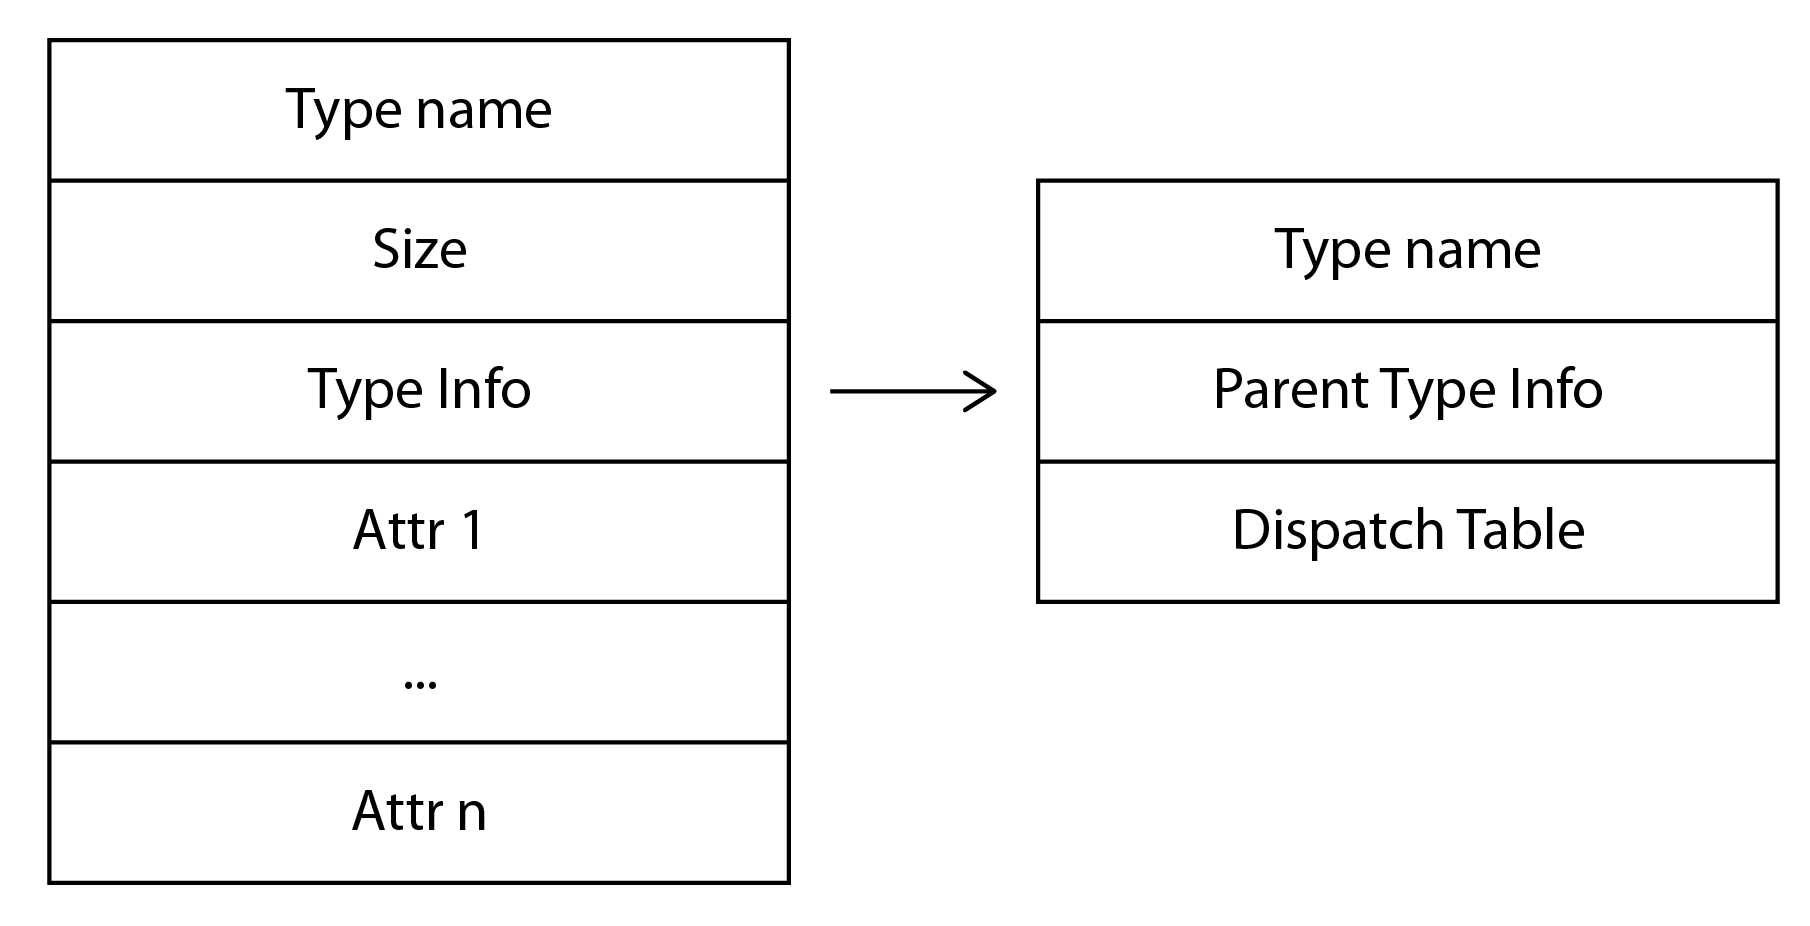
\includegraphics[width=0.6\textwidth]{resources/object.png}
	\label{fig:objects}
	\caption{Representación de los objetos en memoria}
\end{figure}

Cuando se crean los tipos, para cada tipo se crea una tabla de \texttt{Type Info}, que guarda la información de los tipos que se presenta en la parte derecha de la Figura 2.1. \texttt{Type Name} es una referencia al nombre del tipo, y sirve como identificador del mismo, \texttt{Parent Type Info} guarda una referencia a la tabla de tipos del padre, mientras que \texttt{Dispatch Table} tiene una referencia a una tabla en la que están ubicadas, los métodos del objeto tal y como se guardan en CIL: primero los métodos de los padres y luego los de ellos. Los métodos sobreescritos son guardados en la misma posición que ocuparían en el padre. 

Luego, cuando se crea un objeto se calcula para cada uno de ellos el tamaño que ocupará: esto será igual al total de atributos más los 3 campos adicionales usados para guardar información del tipo. En el primer campo se pone el nombre del tipo, luego el tamaño que este ocupa, y después se busca la dirección del \texttt{Type Info} correspondiente al nuevo objeto que se crea. Después son ubicados los atributos primero la del padre y después los definidos por el objeto.

Luego para buscar un atributo se calcula el offset de este atributo en su tipo estático, y este se le sumará más 3 porque ahí es en donde se empiezan a acceder a los atributos. 

Un algoritmo similar es el que se usa para acceder a los métodos: se busca en la posición 3 de la tabla del objeto, donde se obtiene \texttt{Type Info} y desde allí en la posición 3 se accede a la dirección del \texttt{Dispatch Table}, a partir de la cual se busca el índice de la función llamada según la información que se tiene del tipo estático del objeto, luego, esta función es llamada.  Notar que en caso de que su tipo estático no coincida con su tipo dinámico no importa, porque en la dirección buscada estará la verdadera dirección del método. Este puede ser diferente si, por ejemplo, es sobreescrito. A este proceso se le llama \texttt{Dynamic Dispatch}, representado como \texttt{DynamicCallNode} en contraposición con \texttt{StaticCallNode}. En este último se especifica la función a llamar, es decir, no es necesario buscar dinámicamente en la información del objeto, se accede al método de un tipo especificado.

Por otra parte, también requirió especial atención el nodo \texttt{ConformsNode}, usado para determinar si el tipo de una expresión se conforma con un \texttt{typen}. Para calcular esto se accede al \texttt{Type Info} del objeto y a partir de ahí, se realiza un ciclo por los \texttt{Parent Type Info} hasta encontrar alguno que sea igual a \texttt{typen}. La igualdad de tipos se comprueba accediendo a \texttt{Type Name}, como el mismo string es usado para representar este nombre, en el caso de que dicho string coincida con el nombre de \texttt{typen}, entonces se puede decir que los dos tipos son iguales.

Existen otros nodos que hacen uso de esta representación de objetos. \texttt{TypeOfNode}, por ejemplo, devuelve el primer campo del objeto correspondiente al nombre del tipo.

%----------------------------------------------------------------------------------------
%	Problemas técnicos
%----------------------------------------------------------------------------------------

\section{Problemas técnicos y teóricos}

\subsection{Tipos por valor y por referencia}

Una de las problemáticas en el desarrollo del compilador fue la representación de los objetos built-in, en especial: \texttt{Int}, \texttt{Bool} y \texttt{String} que en realidad no son representados como objetos; los dos primeros son tratados por valor mientras el último aunque es por referencia no tiene campos y es guardado en el la sección .data de Mips. Sin embargo, todos son descendientes de \texttt{Object} que es la raíz de todas las clases en COOL y por lo tanto, poseen los métodos que están definidos en ese tipo. Con el objetivo de optimizar la memoria ocupada en el heap estos objetos no son guardados allí y no poseen la estructura de los objetos explicada anteriormente.

Todas estas clases tienen en común que no es posible heredar de ellas, por lo tanto, una variable de tipo \texttt{Int}, \texttt{Bool} y \texttt{String} no es posible que sea otra cosa. Esto permite que no haya problemas a la hora de hacer dispatch: siempre es posible determinar la función a la que se va a llamar, por lo que las funciones de cada uno de estos tipos siempre se llaman estáticamente, determinando el nombre de la función. Los métodos que heredan de Object son redefinidos, ya que estos están implementados teniendo en cuenta la representación de objetos expuesta anteriormente que estos tipos no tienen.

A su vez, se requiere un trato especial en nodos como \texttt{TypeOfNode} porque estas variables no tienen en su primer campo el nombre de su tipo. Para llevar a cabo este análisis se guarda, para cada variable el tipo de dirección a la que hace referencia. Se tienen como tipo de dirección: String, Bool, Int y por Referencia, este último para designar a los objetos representados mediante el modelo de objetos.

Por otro lado, la única manera de tratar algún objeto tipo \texttt{String}, \texttt{Bool} o \texttt{Int} es haciendo un casteo de este objeto de manera indirecta: retornando uno de estos valores cuando el tipo de retorno del método es \texttt{Object} o pasándolos como parámetro cuando el tipo de argumento es \texttt{Object} o de manera general asignándolos a una variable tipo \texttt{Object}. En estos casos se espera que el valor del objeto sea por referencia, así que se hace \textit{Boxing} llevándolos a una representación de objetos, almacenándolos en el heap. Para esto se crea un nodo especial en CIL \texttt{BoxingNode} a partir del cual se llevará a cabo la conversión en Mips. Notar que el proceso contrario \textit{Unboxing} en el que se convierte un objeto por referencia a uno por valor no es necesario implementarlo en COOL: el casteo directo no existe en este lenguaje y asignar un objeto de tipo \texttt{Object} a uno \texttt{Bool}, \texttt{Int} o \texttt{String} consiste un error de tipos.

\subsection{Valor Void en Mips}

Otro de los problemas que se tuvo en cuenta fue la representación del valor nulo en Mips. Para modelar este valor se creo un nuevo tipo, denominado \texttt{Void}, que lo único que contiene es como primer campo el nombre del tipo \texttt{Void}. Para comprobar que un valor es void, por lo tanto, simplemente se comprueba que el nombre del tipo dinámico de una variable sea igual a "texttt{Void}. Los errores de runtime ocasionados por intentar llamar estática o dinámicamente a una variable en void son controlado, así como la evaluación de una expresión en case, que de ser void ocasionaría un error al intentar buscar la información del tipo. Por lo tanto, lo único necesario para la representación de void fue ese campo de nombre del tipo. Comprobar si una expresión por lo tanto consiste solamente en determinar si su tipo es \texttt{Void}.


\begin{itemize}
	\item Hablar de los comentarios y los strings en el lexer.
\end{itemize}

%----------------------------------------------------------------------------------------

\end{document}
